\documentclass[6pt]{article}

\usepackage{tikz}
\usepackage[simplified]{pgf-umlcd}

\usepackage[landscape]{geometry}
\geometry{left=.5in, right=.5in, top=1.3in, bottom=1.3in}

\begin{document}
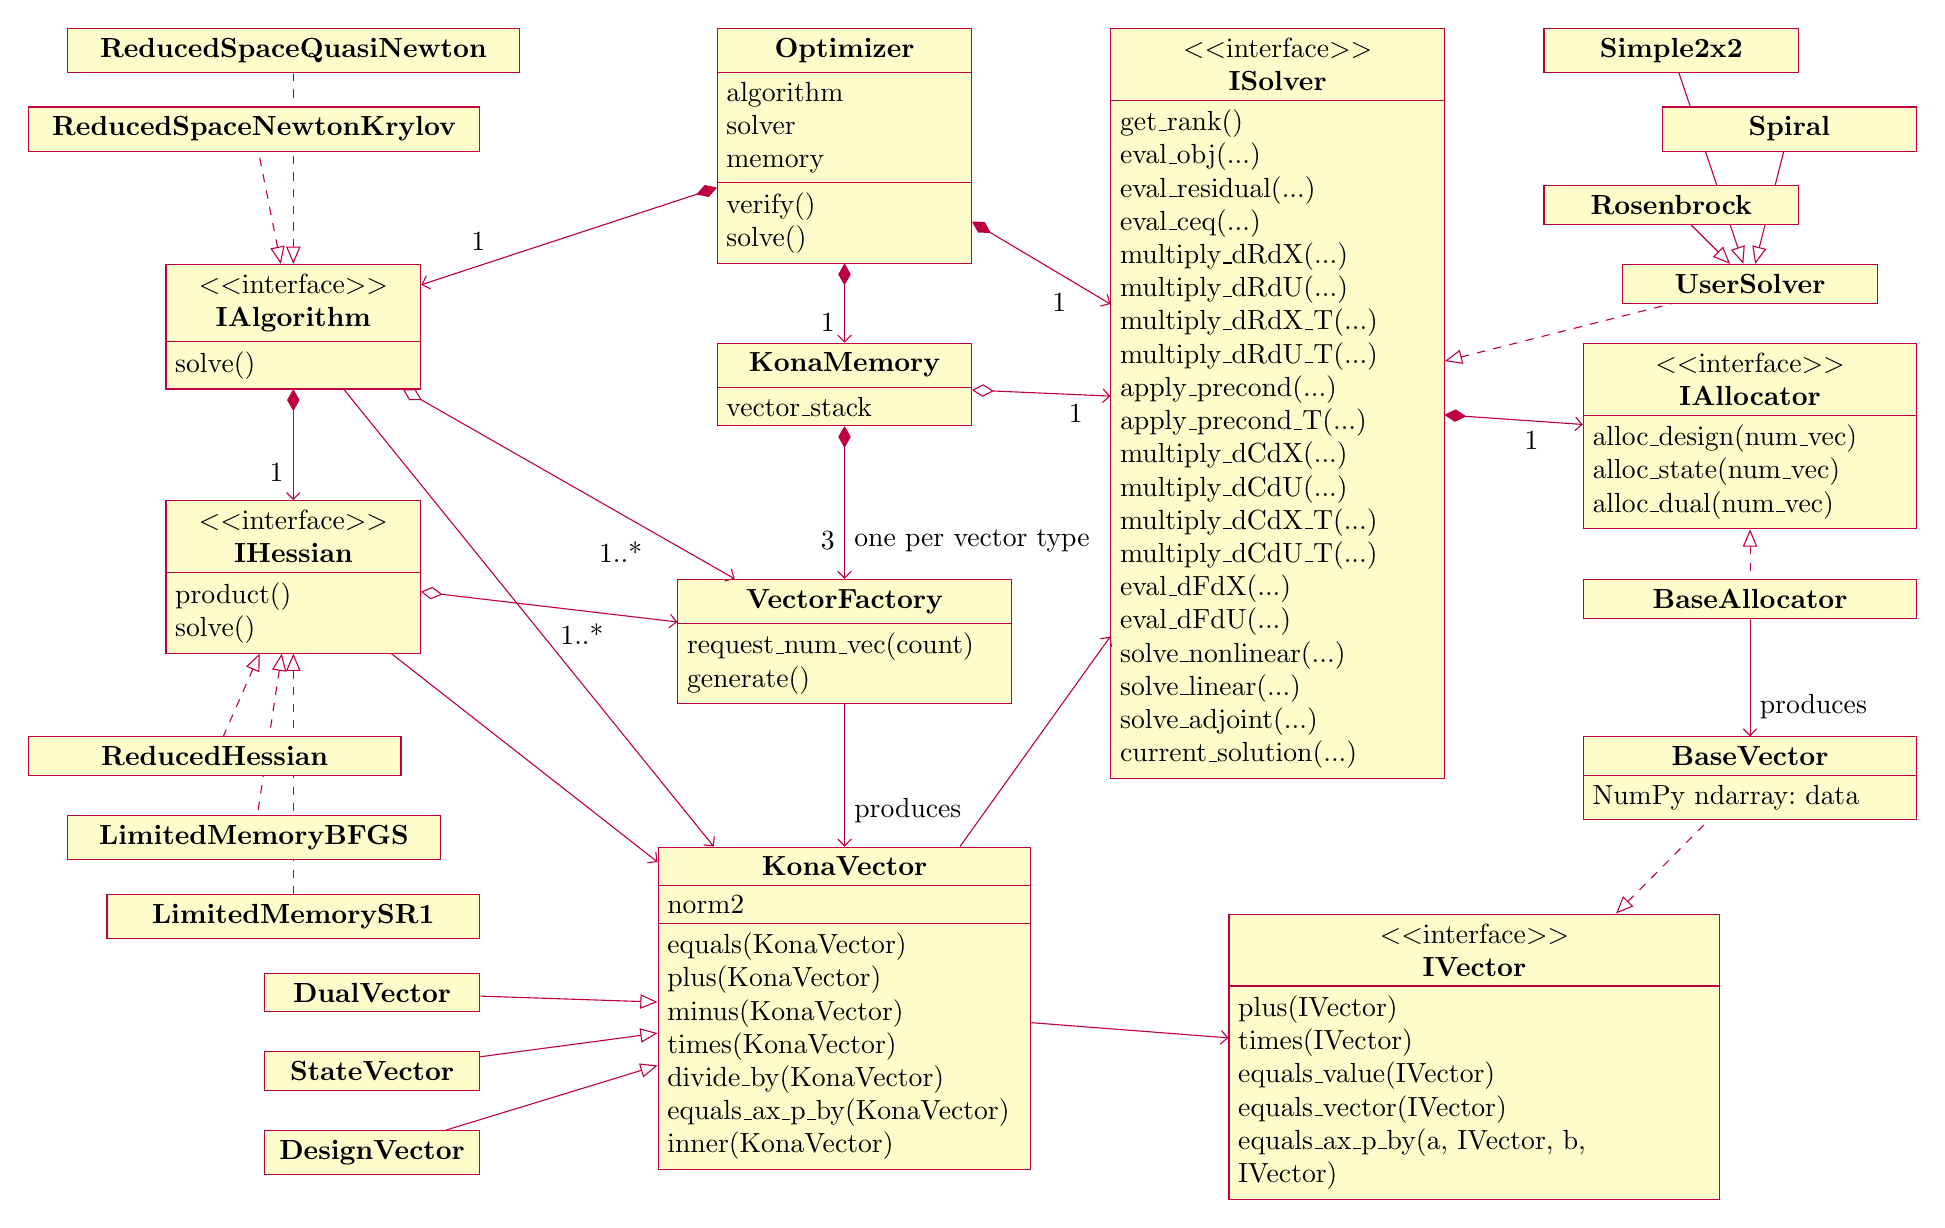
\begin{tikzpicture}[]%[ show background grid ]

	\pagenumbering{gobble}

	% General optimization controller

	\begin{class}[text width = 3cm]{Optimizer}{6,10}
    	\attribute{algorithm}
    	\attribute{solver}
    	\attribute{memory}
		\operation{verify()}
		\operation{solve()}
    \end{class}
    
    % Algorithm interface
    
    \begin{interface}[text width = 3cm]{IAlgorithm}{-1,7}
		\operation{solve()}
    \end{interface}
    
    \begin{class}[text width = 5.5cm]{ReducedSpaceQuasiNewton}{-1,10}
    	\implement{IAlgorithm}	
    \end{class}
    
    \begin{class}[text width = 5.5cm]{ReducedSpaceNewtonKrylov}{-1.5,9}
    	\implement{IAlgorithm}	
    \end{class}
    
    % Hessian interface
    
    \begin{interface}[text width = 3cm]{IHessian}{-1,4}
    	\operation{product()}
    	\operation{solve()}
    \end{interface}
    
    \begin{class}[text width = 4.5cm]{ReducedHessian}{-2,1}
    	\implement{IHessian}	
    \end{class}

	\begin{class}[text width = 4.5cm]{LimitedMemoryBFGS}{-1.5,0}
		\implement{IHessian}	
	\end{class}

	\begin{class}[text width = 4.5cm]{LimitedMemorySR1}{-1,-1}
		\implement{IHessian}	
	\end{class}
	
	% Kona memory manager
	
	\begin{class}[text width = 3cm]{KonaMemory}{6,6}
    	\attribute{vector\_stack}
    \end{class}
    
    % Vector factory
    
    \begin{class}[text width = 4cm]{VectorFactory}{6,3}
        \operation{request\_num\_vec(count)}
        \operation{generate()}
    \end{class}
    
    % Kona vectors
    
    \begin{class}[text width = 4.5 cm]{KonaVector}{6,-0.4}
        \attribute{norm2}
        \operation{equals(KonaVector)}
        \operation{plus(KonaVector)}
        \operation{minus(KonaVector)}
        \operation{times(KonaVector)}
        \operation{divide\_by(KonaVector)}
        \operation{equals\_ax\_p\_by(KonaVector)}
        \operation{inner(KonaVector)}
    \end{class}

    \begin{class}[text width = 2.5 cm]{DesignVector}{0,-4}
        \inherit{KonaVector}
    \end{class}

    \begin{class}[text width = 2.5 cm]{StateVector}{0,-3}
        \inherit{KonaVector}
    \end{class}

    \begin{class}[text width = 2.5 cm]{DualVector}{0,-2}
        \inherit{KonaVector}
    \end{class}
    
    % User solver interface
    
    \begin{interface}[text width = 4cm]{ISolver}{11.5, 10}
    	\operation{get\_rank()}
    	\operation{eval\_obj(...)}
    	\operation{eval\_residual(...)}
    	\operation{eval\_ceq(...)}
    	\operation{multiply\_dRdX(...)}
    	\operation{multiply\_dRdU(...)}
    	\operation{multiply\_dRdX\_T(...)}
    	\operation{multiply\_dRdU\_T(...)}
    	\operation{apply\_precond(...)}
    	\operation{apply\_precond\_T(...)}
    	\operation{multiply\_dCdX(...)}
    	\operation{multiply\_dCdU(...)}
    	\operation{multiply\_dCdX\_T(...)}
    	\operation{multiply\_dCdU\_T(...)}
    	\operation{eval\_dFdX(...)}
    	\operation{eval\_dFdU(...)}
    	\operation{solve\_nonlinear(...)}
    	\operation{solve\_linear(...)}
    	\operation{solve\_adjoint(...)}
    	\operation{current\_solution(...)}
    \end{interface}
    
    \begin{class}[text width = 3cm]{UserSolver}{17.5, 7}
    	\implement{ISolver}	
    \end{class}
    
    \begin{class}[text width = 3cm]{Rosenbrock}{16.5, 8}
    	\inherit{UserSolver}	
    \end{class}
	
	\begin{class}[text width = 3cm]{Spiral}{18, 9}
    	\inherit{UserSolver}	
    \end{class}
    
    \begin{class}[text width = 3cm]{Simple2x2}{16.5, 10}
    	\inherit{UserSolver}	
    \end{class}
    
    % User vector interface

    \begin{interface}[text width = 6cm]{IVector}{14,-1.25}
        \operation{plus(IVector)}
        \operation{times(IVector)}
        \operation{equals\_value(IVector)}
        \operation{equals\_vector(IVector)}
        \operation{equals\_ax\_p\_by(a, IVector, b, IVector)}
    \end{interface}
    
    \begin{class}[text width = 4cm]{BaseVector}{17.5,1}
        \implement{IVector}
        \attribute{NumPy ndarray$\colon$ data}
    \end{class}
    
    % User vector allocator interface

    \begin{interface}[text width = 4cm]{IAllocator}{17.5,6}
        \operation{alloc\_design(num\_vec)}
        \operation{alloc\_state(num\_vec)}
        \operation{alloc\_dual(num\_vec)}
    \end{interface}

    \begin{class}[text width = 4cm]{BaseAllocator}{17.5,3}cd
        \implement{IAllocator}
    \end{class}

    % UML relationships below
    
    \composition{ISolver}{}{1}{IAllocator}
    
    \unidirectionalAssociation{KonaVector}{}{}{ISolver}
    \unidirectionalAssociation{KonaVector}{}{}{IVector}
    
    \aggregation{KonaMemory}{}{1}{ISolver}
    \composition{KonaMemory}{one per vector type}{3}{VectorFactory}
    
    \unidirectionalAssociation{BaseAllocator}{produces}{}{BaseVector}
    
    \unidirectionalAssociation{VectorFactory}{produces}{}{KonaVector}
    
    \composition{Optimizer}{}{1}{IAlgorithm}
    \composition{Optimizer}{}{1}{KonaMemory}
    \composition{Optimizer}{}{1}{ISolver}
    
    \composition{IAlgorithm}{}{1}{IHessian}
    \aggregation{IAlgorithm}{}{1..*}{VectorFactory}
    \unidirectionalAssociation{IAlgorithm}{}{}{KonaVector}
    
    \aggregation{IHessian}{}{1..*}{VectorFactory}
    \unidirectionalAssociation{IHessian}{}{}{KonaVector}

\end{tikzpicture}

\end{document}
